\subsection{Kiến thức về mạng nơron sâu (DNN)}
\subsubsection{mạng nơron sâu thường cho kết quả tốt hơn mạng nơron rộng với cùng số lượng nơron.}

Đối với mạng nơron có N nút, mạng học sâu có số tổ hợp các đường đi nhiều hơn rất nhiều so với mạng học rộng chỉ có một lớp. Nhờ đó các giá trị của hàm xấp xỉ sẽ gần đúng với hàm mục tiêu hơn nên cho kết quả tốt hơn.
\textit{Ví dụ:} Mạng học rộng ở trên chỉ có 6 đường đi khác nhau từ input đến output. Trong khi đó mạng học sâu bên dưới với 3 lớp ẩn có số đường đi khác nhau từ input đến output là 16.
\begin{figure}[H]
	\begin{center}
		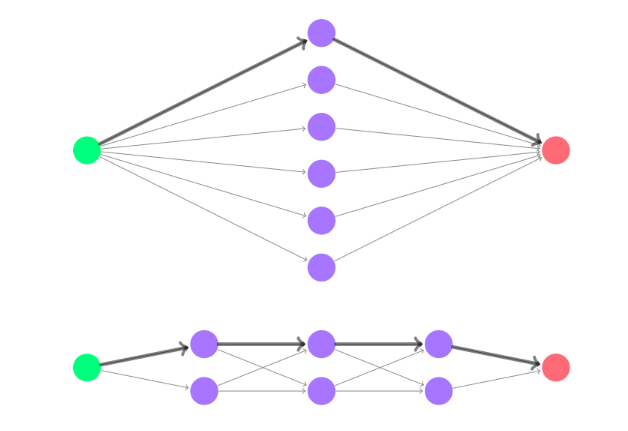
\includegraphics[scale=0.3]{images/theo5/deep-vs-narrow}
		\caption{Lợi ích của mạng học sâu}
	\end{center}
\end{figure} 

\subsubsection{Hàm kích hoạt (Activation functions)}
\begin{enumerate}
	\item \textbf{Sigmoid}
	\begin{itemize}
		\item \textit{Công thức:}
		$$\sigma(x) = \frac{1}{1 + e^{-1}}$$
		\item \textit{Ưu điểm}: hàm sigmoid có đạo hàm đẹp.
		\item \textit{Nhược điểm}: 
		\begin{itemize}
			\item Dễ gây ra các hiện tượng Vanishing / Exploding Gradient khi giá trị đầu vào có trị tuyệt đối quá lớn.
			\item Không có zero-centered, gây ảnh hưởng đến tốt độ hội tụ.
		\end{itemize}
	\end{itemize}
	\item \textbf{ReLU}
	\begin{itemize}
		\item \textit{Công thức:}
		$$ReLU(x) = max(0, x)$$
		\item \textit{Ưu điểm}: 
		\begin{itemize}
			\item Tính toán nhanh và dễ dàng do không sử dụng hàm tính lũy thừa.
			\item Tốt độ hội tụ nhanh.
		\end{itemize}
		\item \textit{Nhược điểm}: các nút có giá trị nhỏ hơn 0 qua hàm ReLU sẽ thành 0. Do đó, thông tin từ nút đấy sẽ không được truyền về cho các nút phía sau.
	\end{itemize}
	\pagebreak

	\item \textbf{Tanh}
	\begin{itemize}
		\item \textit{Công thức:}
		$$tanh(x) = \frac{e^x - e^{-x}}{e^x + e^{-x}}$$
		\item \textit{Ưu điểm}: giống với hàm sigmoid. Hàm tanh có đạo hàm đẹp. Ngoài ra, khác với sigmoid thì hàm tanh có trung tâm là 0 (zero - centered) nhờ đó mà hội tụ tốt hơn sigmoid.
		\item \textit{Nhược điểm}: Hàm tanh có 2 đầu bảo hòa giống với sigmoid. Điều này dẫn đến gradient biến mất hoặc bùng nổ.
	\end{itemize}
\end{enumerate}

\subsubsection{Bộ tối ưu (Optimizer)}
\begin{enumerate}
	\item \textbf{Gradient Descent (GD)}: 
	\begin{itemize}
		\item Tính hàm độ lỗi của toàn bộ dữ liệu huấn luyện. Sau đó tính đạo hàm và tối ưu các tham số tham chiều ngược với đạo hàm.
		\item \textit{Công thức}:
		$$x_{t+1} = x_t + \eta f'(x_t)\text{  ,trong đó $\eta$ là Learning Rate}$$ 
		\item \textit{Ưu điểm: }thuật toán dễ hiểu. Tối ưu được các thao số của mô hình sau các vòng lặp.
		\item \textit{Nhược điểm: }nghiệm tìm được phụ thuộc rất nhiều vào nghiệm khởi tạo ban đầu và learning rate. Các nghiệm khởi tạo khác nhau có thể bị rơi vào các cực trị cục bộ khác nhau và có thể không phải là nghiệm toàn cục. Learning rate quá lớn hoặc quá nhỏ sẽ làm cho quá trình hội tụ diễn ra rất lâu hoặc thậm chí không thể hội tụ. 

	\end{itemize}	
	\item \textbf{Stochastic Gradient Descent (SGD)}
	\begin{itemize}
		\item Sử dụng công thức giống với Gradient Descent. Nhưng ở mỗi epoch, ta cần tính hàm độ lỗi cho một số điểm dữ liệu và cập nhật trọng số.
		\item \textit{Ưu điểm: }đối với tập dữ liệu lớp, GD không thể tính các giá trị như hàm độ lỗi và đạo hàm một cách nhanh chóng. Tuy nhiên đối với SGD thì việc này trở nên dễ dàng.
		\item \textit{Nhược điểm: }giống với GD, SGD chưa giải quyết được vấn đề phụ thuộc và điểm trọng số khởi tạo và learning rate.
	\end{itemize}

	\item \textbf{Momentum}
	\begin{itemize}
		\item Momentum khắc phục nhược điểm của GD và SGD bằng cách thêm một lượng quán tính vào công thức tối ưu tham số. Do đó, dù có đạt đến cực tiểu, các tham số sẽ trượt lên một đoạn để có thể thoát ra khỏi cực trị địa phương hoặc là lăng ngược xuống về điểm cực trị ban đầu.
		\item \textit{Công thức}:
		\begin{align} 
			v_t = \gamma v_{t-1} + \eta f'(x)\\
			\phi = \phi - v_t
		\end{align}
		\item \textit{Ưu điểm: }thuật toán dễ hiểu. Tối ưu được các thao số của mô hình sau các vòng lặp.
		\item \textit{Nhược điểm: }nghiệm tìm được phụ thuộc rất nhiều vào nghiệm khởi tạo ban đầu và learning rate. Các nghiệm khởi tạo khác nhau có thể bị rơi vào các cực trợ cục bộ khác nhau và có thôi không phải là nghiệm toàn cục. learning rate quá lượng hoặc quá nhỏ sẽ làm cho quá trình hội tụ diễn ra rất lâu hoặc thậm chí không thể hội tụ. 
	\end{itemize}
\end{enumerate}

\subsubsection{Drop-out}
\textit{Định nghĩa:} Drop-out là kĩ thuật giúp giảm tỉ lệ overfitting của mạng nơron nhân tạo. Trong khi phương pháp Regulization trước đó đánh phạt cho trọng lượng của các tham số .Drop-out bỏ qua ngẫu nhiên một số nút trong quá trình huấn luyện theo một tỉ lệ 1-p (p được gọi là \textit{Keepting prob}). Nhờ vậy mà một nút mạng không thể phụ thuộc nhiều vào một nút mạng nào đó được (Vì không biết khi nào nút sẽ bị drop-out), từ đó mà độ phụ thuộc (trọng lượng) của các nút liên kết tới sẽ được trải đều, giúp tăng sức mạnh cho các nút mạng trong mạng. 

Hệ số p nên ở khoảng [0.2, 0.5] . Nếu p quá nhỏ thì không có tác dụng chống overfitting, tuy nhiên nếu p quá lớn thì gần như loại bỏ layer đấy và có dễ dẫn đến underfitting.

Drop-out được thực hiên trên tập validation và chia làm 2 giai đoạn:
\begin{itemize}
	\item \textbf{Training}: Với mỗi epoch, với mỗi mini-batch, ta thực hiện drop-out với tỉ lệ drop là (1-p) trên mỗi lớp ẩn.
	\item \textbf{Testing}: Ở giai đoạn testing, ta không thực hiện drop-out trên mạng. Và phải nhân một lượng p vào mỗi tham số để tránh output bị nhân lên gấp đôi.
\end{itemize}
\begin{figure}[H]
	\begin{center}
		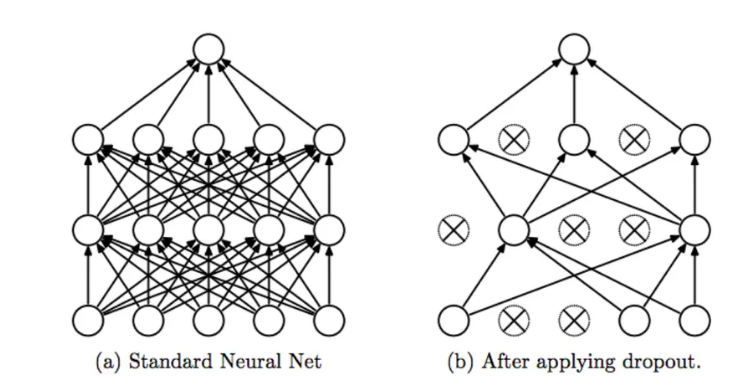
\includegraphics[scale=0.5]{images/theo5/drop-out}
		\caption{Minh họa Drop-out}
	\end{center}
\end{figure}
\pagebreak